\subsection*{Problema 15}

\textbf{Enunciado:}
Calcular la integral indefinida:
\begin{equation*}
\int \dfrac{x^3}{x^2 - 2x - 3} \, dx
\end{equation*}

\textbf{Solución:}
Como el grado del numerador ($3$) es mayor que el grado del denominador ($2$), realizamos primero la división polinómica de $x^3$ entre $x^2 - 2x - 3$.

Dividiendo $x^3$ por $x^2 - 2x - 3$, obtenemos un cociente de $x + 2$ y un residuo de $7x + 6$. Así, el integrando se reescribe como:
\begin{equation*}
\dfrac{x^3}{x^2 - 2x - 3} = x + 2 + \dfrac{7x + 6}{x^2 - 2x - 3}
\end{equation*}

Factorizando el denominador según las indicaciones:
\begin{equation*}
x^2 - 2x - 3 = (x - 3)(x + 1)
\end{equation*}

Aplicamos fracciones parciales al término restante:
\begin{equation*}
\dfrac{7x + 6}{(x - 3)(x + 1)} = \dfrac{A}{x - 3} + \dfrac{B}{x + 1}
\end{equation*}

Multiplicando por el denominador común:
\begin{equation*}
7x + 6 = A(x + 1) + B(x - 3)
\end{equation*}

Si $x = 3$:
\begin{equation*}
7(3) + 6 = A(4) \implies 27 = 4A \implies A = \dfrac{27}{4}
\end{equation*}

Si $x = -1$:
\begin{equation*}
7(-1) + 6 = B(-4) \implies -1 = -4B \implies B = \dfrac{1}{4}
\end{equation*}

Sustituyendo los valores de $A$ y $B$, la integral original se divide en:
\begin{multline*}
\int \dfrac{x^3}{x^2 - 2x - 3} \, dx = \int \left( x + 2 \right) dx \\
+ \int \dfrac{27/4}{x - 3} \, dx + \int \dfrac{1/4}{x + 1} \, dx
\end{multline*}

Integrando cada término por separado, obtenemos la solución general:
\begin{multline*}
\int \dfrac{x^3}{x^2 - 2x - 3} \, dx = \dfrac{x^2}{2} + 2x \\
+ \dfrac{27}{4} \ln|x - 3| + \dfrac{1}{4} \ln|x + 1| + C
\end{multline*}

\begin{figure}[H]
	\centering
	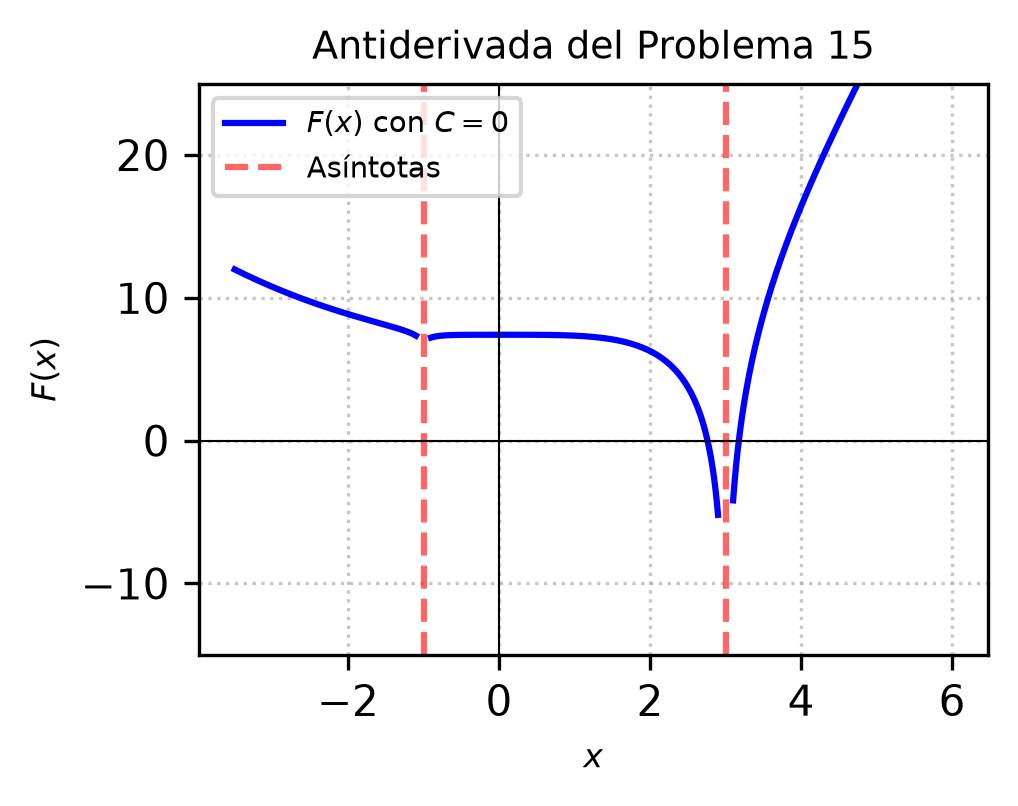
\includegraphics[width=\columnwidth]{semana_03/graficas/SEM03_P15_grafica.png}
	\caption{Representación gráfica de $f(x)$ y su antiderivada $F(x)$ evaluada para la constante de integración $C = 0$ (Problema 15).}
	\label{fig:problema15}
\end{figure}
